\begin{figure}
    % generated by Plantuml 1.2022.5       
    \definecolor{plantucolor0000}{RGB}{255,255,255}
    \definecolor{plantucolor0001}{RGB}{24,24,24}
    \definecolor{plantucolor0002}{RGB}{227,227,227}
    \definecolor{plantucolor0003}{RGB}{0,0,0}
    \definecolor{plantucolor0004}{RGB}{250,250,250}
    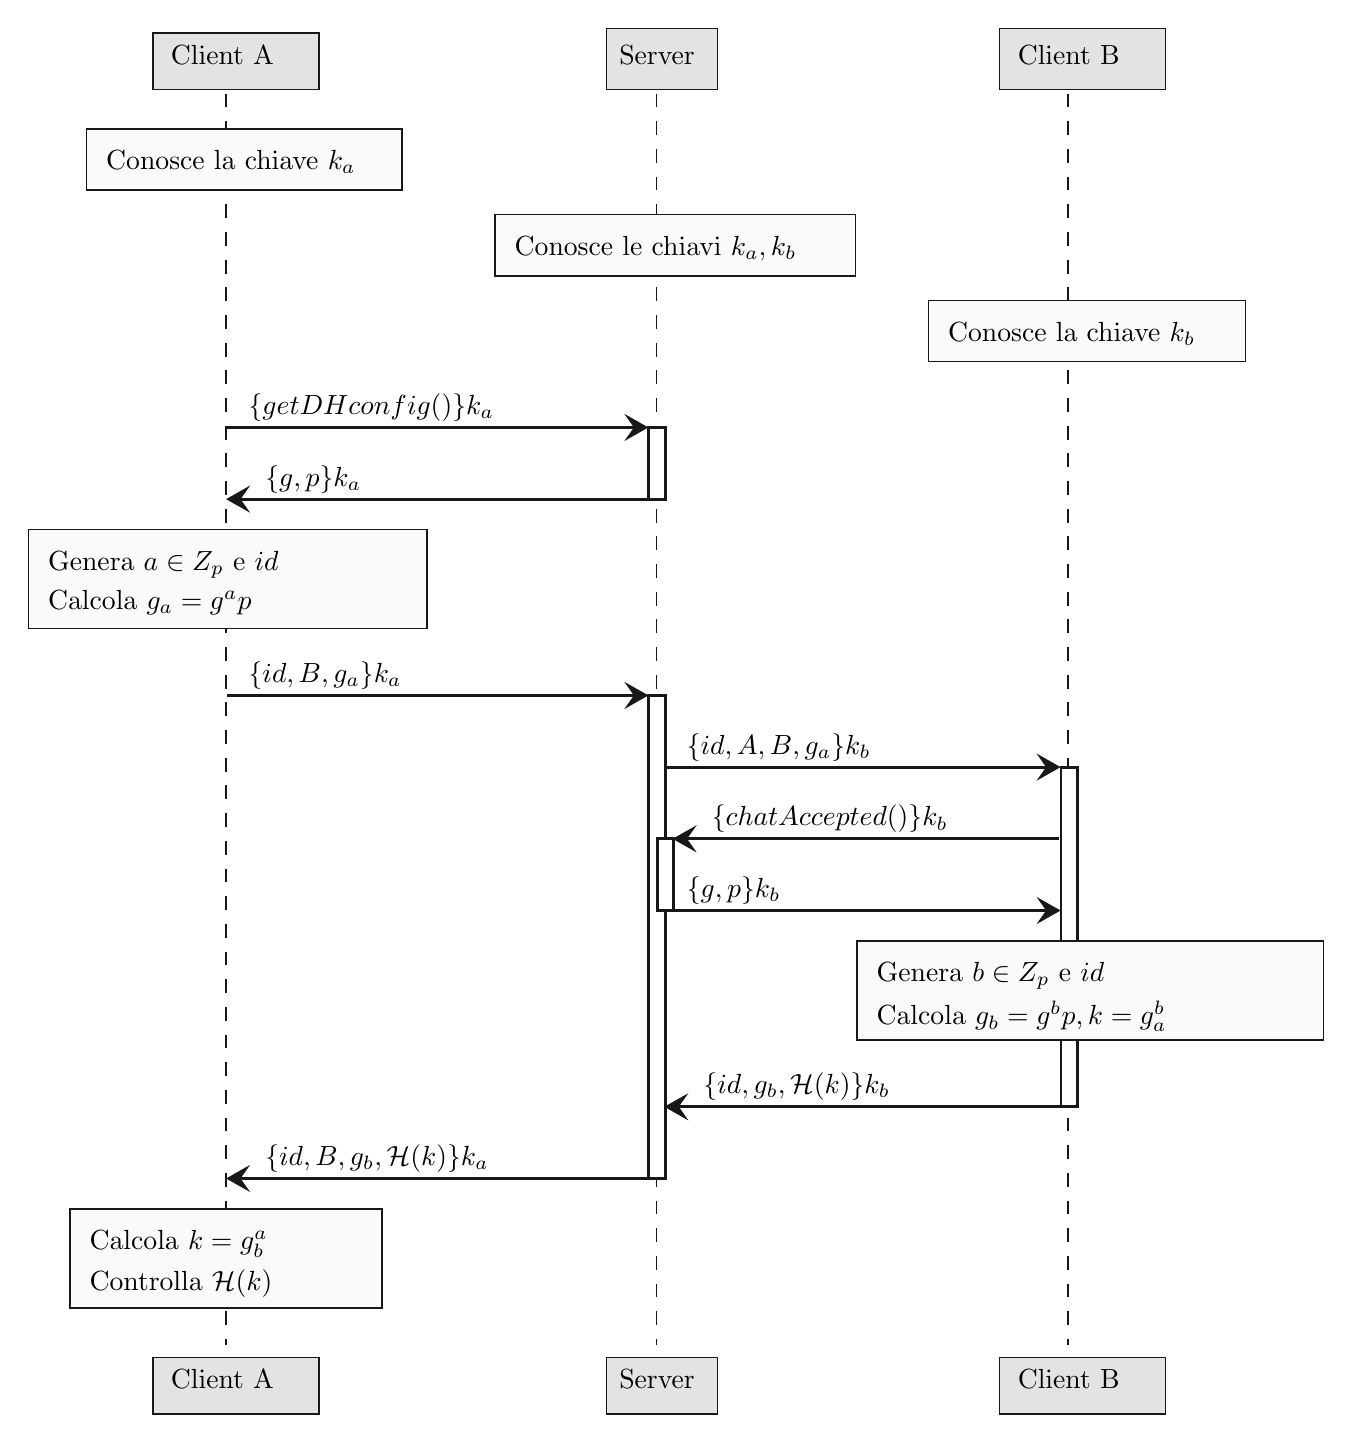
\begin{tikzpicture}[xscale=0.6,yscale=-0.85
            ,pstyle0/.style={color=plantucolor0001,fill=white,line width=1.0pt}
            ,pstyle1/.style={color=plantucolor0001,line width=0.5pt,dash pattern=on 5.0pt off 5.0pt}
            ,pstyle2/.style={color=plantucolor0001,fill=plantucolor0002,line width=0.5pt}
            ,pstyle3/.style={color=plantucolor0001,fill=plantucolor0004,line width=0.5pt}
            ,pstyle4/.style={color=plantucolor0001,fill=plantucolor0001,line width=1.0pt}
            ,pstyle5/.style={color=plantucolor0001,line width=1.0pt}
        ]
        \draw[pstyle0] (378.6934pt,179.6602pt) rectangle (388.6934pt,210.1387pt);
        \draw[pstyle0] (378.6934pt,293.5742pt) rectangle (388.6934pt,498.9238pt);
        \draw[pstyle0] (383.6934pt,354.5313pt) rectangle (393.6934pt,385.0098pt);
        \draw[pstyle0] (626.9471pt,324.0527pt) rectangle (636.9471pt,468.4453pt);
        \draw[pstyle1] (124pt,37.7461pt) -- (124pt,569.8809pt);
        \draw[pstyle1] (383.3042pt,37.7461pt) -- (383.3042pt,569.8809pt);
        \draw[pstyle1] (631.0926pt,37.7461pt) -- (631.0926pt,569.8809pt);

        \draw[pstyle2] (80pt,12pt) rectangle (180pt,36pt);
        \node at (85pt,13pt)[below right,color=black]{Client A};
        \draw[pstyle2] (80pt,575pt) rectangle (180pt,599pt);
        \node at (85pt,576pt)[below right,color=black]{Client A};

        \draw[pstyle2] (353pt,10pt) rectangle (420pt,36pt);
        \node at (355pt,13pt)[below right,color=black]{Server};
        \draw[pstyle2] (353pt,575pt) rectangle (420pt,599pt);
        \node at (355pt,576pt)[below right,color=black]{Server};

        \draw[pstyle2] (590pt,10pt) rectangle (690pt,36pt);
        \node at (595pt,13pt)[below right,color=black]{Client B};
        \draw[pstyle2] (590pt,575pt) rectangle (690pt,599pt);
        \node at (595pt,576pt)[below right,color=black]{Client B};

        \draw[pstyle0] (378.6934pt,179.6602pt) rectangle (388.6934pt,210.1387pt);
        \draw[pstyle0] (378.6934pt,293.5742pt) rectangle (388.6934pt,498.9238pt);
        \draw[pstyle0] (383.6934pt,354.5313pt) rectangle (393.6934pt,385.0098pt);
        \draw[pstyle0] (626.9471pt,324.0527pt) rectangle (636.9471pt,468.4453pt);
        \draw[pstyle3] (40pt,52.7461pt) rectangle (230pt,78.7461pt);
        \node at (46pt,57.7461pt)[below right,color=black]{Conosce la chiave $k_a$};
        \draw[pstyle3] (286pt,89.2246pt) rectangle (503pt,115.2246pt);
        \node at (292pt,94.2246pt)[below right,color=black]{Conosce le chiavi $k_a, k_b$};
        \draw[pstyle3] (547pt,125.7031pt) rectangle (738pt,151.7031pt);
        \node at (553pt,130.7031pt)[below right,color=black]{Conosce la chiave $k_b$};
        \draw[pstyle4] (366.6934pt,175.6602pt) -- (376.6934pt,179.6602pt) -- (366.6934pt,183.6602pt) -- (370.6934pt,179.6602pt) -- cycle;
        \draw[pstyle5] (124.7778pt,179.6602pt) -- (372.6934pt,179.6602pt);
        \node at (131.7778pt,161.1816pt)[below right,color=black]{$\{getDHconfig()\}k_a$};
        \draw[pstyle4] (135.7778pt,206.1387pt) -- (125.7778pt,210.1387pt) -- (135.7778pt,214.1387pt) -- (131.7778pt,210.1387pt) -- cycle;
        \draw[pstyle5] (129.7778pt,210.1387pt) -- (382.6934pt,210.1387pt);
        \node at (141.7778pt,191.6602pt)[below right,color=black]{$\{g, p\}k_a$};
        \draw[pstyle3] (5pt,223.1387pt) rectangle (245pt,265.1387pt);
        \node at (11pt,228.1387pt)[below right,color=black]{Genera $a \in \mathbb{Z}_p$ e $id$};
        \node at (11pt,244.6172pt)[below right,color=black]{Calcola $g_a = g^a \mod p$};
        \draw[pstyle4] (366.6934pt,289.5742pt) -- (376.6934pt,293.5742pt) -- (366.6934pt,297.5742pt) -- (370.6934pt,293.5742pt) -- cycle;
        \draw[pstyle5] (124.7778pt,293.5742pt) -- (372.6934pt,293.5742pt);
        \node at (131.7778pt,275.0957pt)[below right,color=black]{$\{id, B, g_a\}k_a$};
        \draw[pstyle4] (614.9471pt,320.0527pt) -- (624.9471pt,324.0527pt) -- (614.9471pt,328.0527pt) -- (618.9471pt,324.0527pt) -- cycle;
        \draw[pstyle5] (388.6934pt,324.0527pt) -- (620.9471pt,324.0527pt);
        \node at (395.6934pt,305.5742pt)[below right,color=black]{$\{id, A, B, g_a\}k_b$};
        \draw[pstyle4] (404.6934pt,350.5313pt) -- (394.6934pt,354.5313pt) -- (404.6934pt,358.5313pt) -- (400.6934pt,354.5313pt) -- cycle;
        \draw[pstyle5] (398.6934pt,354.5313pt) -- (625.9471pt,354.5313pt);
        \node at (410.6934pt,336.0527pt)[below right,color=black]{$\{chatAccepted()\}k_b$};
        \draw[pstyle4] (614.9471pt,381.0098pt) -- (624.9471pt,385.0098pt) -- (614.9471pt,389.0098pt) -- (618.9471pt,385.0098pt) -- cycle;
        \draw[pstyle5] (388.6934pt,385.0098pt) -- (620.9471pt,385.0098pt);
        \node at (395.6934pt,366.5313pt)[below right,color=black]{$\{g, p\}k_b$};
        \draw[pstyle3] (504pt,398.0098pt) rectangle (785pt,440.0098pt);
        \node at (510pt,403.0098pt)[below right,color=black]{Genera $b \in \mathbb{Z}_p$ e $id$};
        \node at (510pt,419.4883pt)[below right,color=black]{Calcola $g_b = g^b \mod p, k = g_a^b$};
        \draw[pstyle4] (399.6934pt,464.4453pt) -- (389.6934pt,468.4453pt) -- (399.6934pt,472.4453pt) -- (395.6934pt,468.4453pt) -- cycle;
        \draw[pstyle5] (393.6934pt,468.4453pt) -- (630.9471pt,468.4453pt);
        \node at (405.6934pt,449.9668pt)[below right,color=black]{$\{id, g_b, \mathcal{H}(k)\}k_b$};
        \draw[pstyle4] (135.7778pt,494.9238pt) -- (125.7778pt,498.9238pt) -- (135.7778pt,502.9238pt) -- (131.7778pt,498.9238pt) -- cycle;
        \draw[pstyle5] (129.7778pt,498.9238pt) -- (382.6934pt,498.9238pt);
        \node at (141.7778pt,480.4453pt)[below right,color=black]{$\{id, B, g_b, \mathcal{H}(k)\}k_a$};
        \draw[pstyle3] (30pt,511.9238pt) rectangle (218pt,553.9238pt);
        \node at (36pt,516.9238pt)[below right,color=black]{Calcola $k = g_b^a$};
        \node at (36pt,533.4023pt)[below right,color=black]{Controlla $\mathcal{H}(k)$};
    \end{tikzpicture}
    \caption{Diagramma di sequenza della creazione di chat segrete con crittografia \gls{e2e} in \gls{mtproto}.
        La funzione hash $\mathcal{H}$ è SHA1.} \label{fig:mtproto-sequence-secret-chat}
\end{figure}
